\documentclass[11pt,a4paper]{article}
\usepackage[T1]{fontenc}
\usepackage[utf8]{inputenc}
\usepackage[margin=2cm,includefoot,footskip=30pt]{geometry}
\usepackage{amsmath}
\usepackage{amssymb}
\usepackage{helvet}
\usepackage{graphicx}
\usepackage[dvipsnames]{xcolor}
\usepackage{pgfgantt}
\usepackage{parskip}
\usepackage[hidelinks]{hyperref}
\usepackage[polish]{babel}
\usepackage{float}

\renewcommand{\familydefault}{\sfdefault}
\renewcommand{\arraystretch}{1.5}

\begin{document}

    \begin{titlepage}
        \centering
        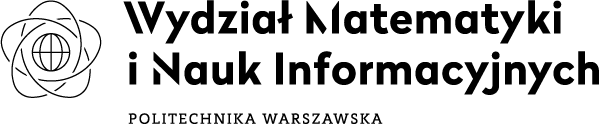
\includegraphics[width=\textwidth]{resources/WMiNI-znak-black.png} \par
        \vspace{3cm}
        {\LARGE Programy działań z efektami domyślnymi \par}
        \vspace{0.5cm}
        {\Large Reprezentacja Wiedzy - projekt \par}
        \vspace{2cm}
        {\large     	
            Bartosz Borkowicz \\
            Sebastian Konowrocki \\
            Tomasz Laskowski \\
            Piotr Łazarczyk \\
            Jakub Niemyjski \\
           	Bartłomiej Pieńkowski \\
            Igor Pieńkowski \\
            Bartłomiej Teodorczuk \\
            Łukasz Wasilewski
        \par}
        \vspace{4cm}
        {\large Wersja 1.0 \par}
        \vspace{0.5cm}
        {\large \today \par}
    \end{titlepage}

    \tableofcontents
    \newpage

    \section{Opis zadania}

	\section{Język akcji}
	
    \subsection{Sygnatura}
    
    \subsection{Syntaktyka}
    
    \subsection{Semantyka}
    
    \section{Język kwerend}
    
    \subsection{Syntaktyka}
    
    \subsection{Semantyka}
    
    \section{Przykłady}
    
\end{document}